\documentclass[a4paper,12pt]{article}

\usepackage{mystyle}

\usepackage{gensymb}
\usepackage{scalerel}
\usepackage{stackengine}

% \usepackage{skull}  % skull
\usepackage{halloweenmath}  % \bigpumpkin, skull (https://tug.ctan.org/info/symbols/comprehensive/symbols-a4.pdf -- Table 76)


\graphicspath{ {images/} }


% https://tex.stackexchange.com/questions/5461/is-it-possible-to-change-the-size-of-an-arrowhead-in-tikz-pgf
\usetikzlibrary{arrows.meta}


\DeclareMathOperator{\Image}{Im}

\definecolor{pink}{RGB}{218, 3, 174}
\definecolor{violet}{RGB}{148, 0, 211}
\definecolor{green}{RGB}{0, 153, 0}
\definecolor{orange}{RGB}{255, 153, 0}
\definecolor{blue}{RGB}{5, 73, 255}
\definecolor{cyan}{RGB}{31, 206, 203}
\definecolor{cyan2}{RGB}{0, 166, 147}
\definecolor{cyangreen}{RGB}{0, 155, 118}
\definecolor{cyangreen2}{RGB}{0, 109, 91}


% https://tex.stackexchange.com/a/101138/135045

\newcommand\widesim[1]{\ThisStyle{%
  \setbox0=\hbox{$\SavedStyle#1$}%
  \stackengine{-.1\LMpt}{$\SavedStyle#1$}{%
    \stretchto{\scaleto{\SavedStyle\mkern.2mu\sim}{.5150\wd0}}{.6\ht0}%
  }{O}{c}{F}{T}{S}%
}}


\newcommand{\BigMiddleThree}{\;\left|\vphantom{\begin{pmatrix} 0\\0\\0 \end{pmatrix}}\right.\;}
\newcommand{\BigMiddleFour}{\;\left|\vphantom{\begin{pmatrix} 0\\0\\0\\0 \end{pmatrix}}\right.\;}


% https://tex.stackexchange.com/questions/63531/how-to-write-quotation-marks-in-math-environment
\DeclareMathSymbol{\mlq}{\mathord}{operators}{``}
\DeclareMathSymbol{\mrq}{\mathord}{operators}{`'}


\DeclareMathOperator{\Imag}{Im}


% https://tex.stackexchange.com/questions/544453/undefined-control-sequence-after-paragraph
\renewcommand{\paragraph}[1]{\noindent\textbf{#1}\quad}


% https://tex.stackexchange.com/questions/36851/skipping-line-after-proof-in-proof-environment#comment73553_36851
\newcommand{\proofindent}{\hspace*{\fill}\par\vspace{0.5em}\noindent}


% https://tex.stackexchange.com/questions/4813/extendible-equals-sign
\makeatletter
\newcommand*{\Relbarfill@}{\arrowfill@\Relbar\Relbar\Relbar}
\newcommand*{\xeq}[2][]{\ext@arrow 0055\Relbarfill@{#1}{#2}}
\makeatother


% https://tex.stackexchange.com/questions/279100/typeset-the-shrug-%C2%AF-%E3%83%84-%C2%AF-emoji
\newcommand{\shrug}[1][]{%
\begin{tikzpicture}[baseline,x=0.8\ht\strutbox,y=0.8\ht\strutbox,line width=0.125ex,#1]
  \def\arm{(-2.5,0.95) to (-2,0.95) (-1.9,1) to (-1.5,0) (-1.35,0) to (-0.8,0)};
  \draw \arm;
  \draw[xscale=-1] \arm;
  \def\headpart{(0.6,0) arc[start angle=-40, end angle=40,x radius=0.6,y radius=0.8]};
  \draw \headpart;
  \draw[xscale=-1] \headpart;
  \def\eye{(-0.075,0.15) .. controls (0.02,0) .. (0.075,-0.15)};
  \draw[shift={(-0.3,0.8)}] \eye;
  \draw[shift={(0,0.85)}] \eye;
  % draw mouth
  \draw (-0.1,0.2) to [out=15,in=-100] (0.4,0.95); 
\end{tikzpicture}}



% https://tex.stackexchange.com/a/314638/135045
\newcommand{\diff}{\mathop{}\!d\!}



\author{Алексеев Василий}


\title{Семинар 4 + 5}
\date{23 + 30 сентября 2024}


\begin{document}
  \maketitle
  
  \tableofcontents

  \thispagestyle{empty}
  
  \newpage
  
  
  
  \vspace*{\fill}
  
  \noindent
  \emph{
    К формулировкам и доказательствам (если такие вообще приводятся) стоит относиться критически.
    Основное в этом конспекте~---~решение задач (но ``критичность'' и здесь лучше не отключать).
    За строгой, ясной и последовательной теорией лучше обращаться к ``нормальным'' источникам.
    (Например, к лекциям.)
  }
  
  \vspace*{\fill}
  
  \thispagestyle{empty}
  
  \newpage
  
  
  \pagenumbering{arabic}


  \section{Функции}
  
  %\begin{figure}[ht]
    %\centering
    %\includegraphics[width=0.6\linewidth]{images/Apples}
    %
    %\caption{
      %Одно яблоко, два яблока, ...~---~натуральные числа используются при счёте предметов.
    %}
    %\label{fig:naturals}
  %\end{figure}


  % TODO: про инъективность, сюръективность
  
  

  \section{Предел функции}

  % Определения
  % Односторонние пределы
  % Эквивалентные
  % О-малое
  % Замечательные пределы
  %   Про смысл первого и второго
  % Свойства (предел сложной функции)


  \section{Непрерывность функции}

  % Определение
  % Критерий Коши существования конечного предела (?)
  % Типы точек разрыва
  % Теорема о достижении точных верхней и нижней граней
  % Теорема о промежуточных значениях (задача)
  



  \subsection{С1, \S 9, \textnumero 20(2)}

  Найти предел функции:
  \[
    \lim_{x \to 1} \frac{x^2 + 4x - 5}{x^2 - 1}
  \]
  
  \begin{solution}
    Имеем неопределённость (вида $0 \hm/ 0$), поэтому пока ``просто подставить'' значение в формулу не получится.
    Но видно, что можно разложить на множители знаменатель (и числитель)~---~возможно, ``проблемность'' сократится:
    \[
      \lim_{x \to 1} \frac{x^2 + 4x - 5}{x^2 - 1}
        = \lim_{x \to 1} \frac{(x - 1) (x + 5)}{(x - 1) (x + 1)}
        = \lim_{x \to 1} \frac{x + 5}{x + 1}
        = \frac{6}{2} = 3
    \]
    То, на что сокращали~---~это не ноль! потому что $x$ \emph{стремится} к $1$, то есть подходит всё ближе и ближе к единице, никогда в неё не попадая, и потому выражение $x \hm- 1$ \emph{стремится} к нулю, но никогда нулю не равно.
    А в конце, когда ``проблема'' ушла, уже можно было просто ``подставить'' в формулу значение $x \hm= 1$.
  \end{solution}


  \subsection{С1, \S 9, \textnumero 25(5)}

  Найти предел функции:
  \[
    \lim_{x \to 5} \frac{\sqrt{6 - x} - 1}{3 - \sqrt{4 + x}}
  \]
  
  \begin{solution}
    Снова неопределённость ($0 \hm/ 0$).
    В данном случае же, очевидно, на множители ничего не раскладывается.
    Однако можно воспользоваться другим приёмом~---~``домножить и поделить'':
    \begin{equation*}
    \begin{split}
      \lim_{x \to 5} \frac{\sqrt{6 - x} - 1}{3 - \sqrt{4 + x}}
        &= \lim_{x \to 5} \frac{\left(\sqrt{6 - x} - 1\right) \textcolor{blue}{\left(\sqrt{6 - x} + 1\right)} \textcolor{pink}{\left(3 + \sqrt{4 + x}\right)}}{\left(3 - \sqrt{4 + x}\right) \textcolor{pink}{\left(3 + \sqrt{4 + x}\right)} \textcolor{blue}{\left(\sqrt{6 - x} + 1\right)}}\\
        &= \lim_{x \to 5} \frac{(5 - x) \left(3 + \sqrt{4 + x}\right)}{(5 - x) \left(\sqrt{6 - x} + 1\right)}
        = \lim_{x \to 5} \frac{3 + \sqrt{4 + x}}{\sqrt{6 - x} + 1}
        = \left.\frac{3 + \sqrt{4 + x}}{\sqrt{6 - x} + 1}\right|_{x = 5}
        = 3
    \end{split}
    \end{equation*}
    В итоге снова почти-равный-но-до-конца-не-равный нулю множитель сократился, и неопределённости после этого уже не было.
  \end{solution}


  \subsection{С1, \S 9, \textnumero 30(2)}

  Найти предел функции:
  \[
    \lim_{x \to \pi} \frac{\sin x}{\pi^2 - x^2}
  \]

  \begin{solution}
    Видно, что предел ``похож'' на первый замечательный.  % TODO: ref
    (И кроме как сведения к первому замечательному не понятно, как его вообще находить.)
    Поэтому попробуем ``выделить'' в явном виде этот табличный предел, немного повертев выражение, задающее функцию:
    \begin{equation*}
    \begin{split}
      \lim_{x \to \pi} \frac{\sin x}{\pi^2 - x^2}
        &= \lim_{x \to \pi} \frac{\sin x}{(\pi - x) (\pi + x)}\\
        &= \lim_{x \to \pi} \frac{\sin{(\pi - x)}}{(\pi - x) (\pi + x)}
        = \lim_{x \to \pi} \frac{\textcolor{pink}{\sin{(\pi - x)}}}{\textcolor{pink}{(\pi - x)} (\pi + x)}
        = \blacktriangle
    \end{split}
    \end{equation*}

    Теперь первый замечательный предел виден.
    Это в самом деле он, так как при $x \hm\to \pi$ имеем $(\pi \hm- x) \hm\to 0$.
    Можно сделать замену, чтоб совсем было один-в-один по виду, как в замечательном:
    \[
      \pi - x \equiv t,\quad x = \pi + t,\quad x \to \pi \Leftrightarrow t \to 0
    \]

    Тогда, возвращаясь к пределу:
    \[
      \blacktriangle = \lim_{t \to 0} \frac{\sin t}{t} \frac{1}{2 \pi + t}
        = \frac{1}{2 \pi}
    \]
  \end{solution}


  \subsection{С1, \S 9, \textnumero 36(2)}

  Найти предел функции:
  \[
    \lim_{x \to 0} \left(\sqrt{1 + x} - x\right)^{1 / x}
  \]

  \begin{solution}
    А этот предел чем-то напоминает второй замечательный.  % TODO: ref
    Поэтому снова попробуем немного ``причесать'' функцию под пределом.
    Так как
    \[
      \sqrt{1 + x} = (1 + x)^{1/2}
    \]
    то можно воспользоваться следующим равенством:
    \[
      \sqrt{1 + x} = 1 + \frac{1}{2}\, x + o(x),\quad x \to 0
    \]

    Подставим это в предел:
    \[
      \lim_{x \to 0} \left(\sqrt{1 + x} - x\right)^{1 / x}
        = \lim_{x \to 0} \left(1 + \frac{1}{2}\, x - x + o(x)\right)^{1 / x}
        = \lim_{x \to 0} \left(1 - \frac{1}{2}\, x + o(x)\right)^{1 / x}
        = \blacktriangle
    \]

    $o(x)$~---~это какая-то функция, бесконечно малая\footnote{
      Дающая в пределе ноль (а не ``минус бесконечность'').
    } по отношению к функции~$x$ при $x \hm\to 0$.
    Так как в той же скобке присутствует ещё и сам $x$ (с коэффициентом $-1\hm/2$), то на $o(x)$ можно смотреть как ``практически'' на ноль (это поправка, которая несравнимо меньше члена $-x\hm/2$ по величине).
    Другими словами, можно просто ``забыть'' про $o(x)$:\footnote{
      ``Забывать'' можно не всегда, а только тогда, когда это в самом деле ``бесконечно малая'' поправка, по сравнению с другими членами. 
      Например, в пределе $\lim_{x \to 0} \left(1 + x^2\right)^{1/x^2}$ функция $x^2$ тоже будет $o(x)$, но ``отметание'' её в сумме в скобке приведёт к приделу $\lim_{x \to 0} 1^{1/x^2}$.
      Который, очевидно, не равен исходному.
      Бывают также случаи, когда... не только не стоит ``отметать'' поправку, а когда, наоборот, необходимо её как-то уточнить, разложить до ещё большей точности.
      Например, пусть есть предел $\lim_{x \to 0} \left(\sqrt{1 + x} \hm- x \hm/ 2\right)^{1/x^2}$.
      Раскладывая до $o(x)$ корень, переходим к пределу $\lim_{x \to 0} \left(1 \hm+ o(x)\right)^{1/x^2}$, с которым уже и не понятно, что делать.
      Потому что выкинуть $o(x)$ нельзя: она хоть и малая, но играет роль.
      Например, вместо $o(x)$ могла бы быть, например, функция $x^2$, или $-17{.}5 x^2$, или $x^{2024}$~---~итоговый ответ в каждом из случаев был бы другим.
      Таким образом, в данном примере нужно бы было каким-то образом раскладывать корень не до $o(x)$, а до какой-то более высокой точности (до ещё более малой поправки)...
    }
    \[
      \blacktriangle = \lim_{x \to 0} \left(1 - \frac{x}{2}\right)^{\frac{1}{x}} = \spadesuit
    \]

    Второй замечательный предел почти проявился, правда, ещё не до конца...
    Но его можно получить, если теперь ``домножить и поделить'' в степени:
    \[
      \spadesuit = \lim_{x \to 0} \left(1 - \frac{x}{2}\right)^{\frac{2}{x} \cdot \frac{1}{2}}
        = e^{1/2} = \sqrt{e}
    \]
    (По ходу пользовались тем, что $x \hm/ 2 \hm\to 0$ при $x \hm\to 0$.
    Можно бы было сделать замену, чтоб получить второй замечательный предел прям в как в табличном виде.
    Но можно было и просто иметь это в виду (делая ``мысленную замену'').)
  \end{solution}


  \subsection{С1, \S 9, \textnumero 61}

  Пусть известно, что
  \[
    \begin{aligned}
      &\lim_{y \to y_0} f(y) = a\\
      &\lim_{x \to x_0} g(x) = y_0
    \end{aligned}
  \]

  Следует ли отсюда, что
  \[
    \lim_{x \to x_0} f\bigl(g(x)\bigr) = \lim_{y \to y_0} f(y) = a
  \]
  
  \begin{solution}
    Очевидно, условие задачи представляет ``практически'' утверждение о непрерывности сложной функции.  % TODO: ref
    С тем отличием, что не требуется, чтобы $g(x) \hm{\not=} y_0$ хотя бы в некоторой $\delta$-окрестности $x_0$.
    Таким образом, при взятии предела
    \[
      \lim_{x \to x_0} f\bigl(g(x)\bigr)
    \]
    может получиться так, что при стремлении $x \to x_0$ функция $g(x)$ пройдёт через $y_0$.
    Но ведь при рассмотрении предела
    \[
      \lim_{y \to y_0} f(y)
    \]
    вообще не важно, что происходит с $f(y)$ в самой точке~$y_0$ (функция $f(y)$ может быть даже не определена в ней).
    Отсюда и может возникнуть противоречие: с $f(y)$ что-то ``нехорошо'' в самой $y_0$, а $g(x)$ в неё попадает при $x \hm\to x_0$ (функция $g(x)$ в любом случае \emph{стремится} к $y_0$ при $x \hm\to x_0$~---~тут же важно, что она может именно пройти через $y_0$, принять это значение~---~не в пределе).

    Наверняка можно придумать не один (контр)пример, решающий задачу...

    Как вариант, предлагается завязаться снова на замечательный предел (первый).
    Рассмотрим ситуацию:
    \[
      f(y) = \frac{\sin y}{y}, \quad g(x) = 0
    \]
    то есть $g(x)$ просто константный ноль; в качестве же $y_0$, очевидно, берём $y_0 \hm= 0$;
    точка же $x_0$ может быть любой, пусть, для определённости, тоже $x_0 \hm= 0$.
    Тогда получаем
    \[
      \left\{\begin{aligned}
        &\lim_{y \to y_0} f(y) = \lim_{y \to 0} \frac{\sin y}{y} = 1\\
        &\lim_{x \to x_0} g(x) = \lim_{x \to 0} 0 = 0
      \end{aligned}\right.
    \]

    Однако
    \[
      \lim_{x \to x_0} f\bigl(g(x)\bigr) = \lim_{x \to 0} \frac{\sin 0}{0} \quad (\pumpkin)
    \]

    Получили в явном виде деление на ноль.
    Дальнейшие объяснения кажутся излишними.\footnote{
      Всё-таки на всякий случай ещё одно небольшое замечание: в первом замечательном пределе $\lim_{x \to 0} \frac{\sin x}{x}$ нет деления на ноль! ноль никогда не возникает в знаменателе (при $x \hm\to 0$ знаменатель становится \emph{всё ближе} к нулю, бесконечно близко, но всё-таки не ``чистый'' ноль).
    }
  \end{solution}


  %% DAY 2

  % \subsection{С1, \S 7, \textnumero 218(5)}  % График sin(1/x)
  % \begin{solution}
  % \end{solution}


  % Номер-вспоминание
  \subsection{С1, \S 9, \textnumero 36(8)}

  Найти предел функции:
  \[
    \lim_{x \to 0} \bigl(\ln(e + x)\bigr)^{\ctg x}
  \]
  
  \begin{solution}
    Попытаемся постепенно прийти ко второму замечательному пределу:
    \[
      \lim_{x \to 0} \bigl(\ln(e + x)\bigr)^{\ctg x}
        = \lim_{x \to 0} \left(\ln\left\{ e \left(1 + \frac{x}{e}\right) \right\}\right)^{\ctg x}
        = \lim_{x \to 0} \left(1 + \ln\left\{1 + \frac{x}{e}\right\}\right)^{\ctg x}
        = \blacktriangle
    \]

    Воспользуемся равенствами при $x \to 0$:
    \[
      \left\{
        \begin{aligned}
          &\ln\left(1 + \frac{x}{e}\right) = \frac{x}{e} + o(x)\\
          &\ctg x = \frac{1}{\tg x} = \frac{1}{x + o(x)} \sim \frac{1}{x}
        \end{aligned}
      \right.
    \]

    Подставляя в формулу для предела:
    \[
      \blacktriangle = \lim_{x \to 0} \left(1 + \frac{x}{e} + o(x)\right)^{\frac{1}{x}} = \diamondsuit
    \]

    ``Забывая'' про $o(x)$ и ``подкручивая'' (в рамках правил) степень, наконец получаем замечательный предел:
    \[
      \diamondsuit = \lim_{x \to 0} \left(1 + \frac{x}{e}\right)^{\frac{e}{x} \cdot \frac{1}{e}}
        = e^{1/e}
    \]
  \end{solution}
 

  \subsection{С1, \S 10, \textnumero 5(9)}

  Доказать (по определению), что функция $y(x)$ непрерывна в каждой точке своей области определения:
  \[
    y(x) = \frac{1}{x^2}
  \]
  
  \begin{solution}
    % TODO Два способа (два определения)
    Область определения: $\RR \hm\setminus \{0\}$.
    Пусть есть $x_0 \hm{\not=} 0$.
    Покажем, что $f(x)$ непрерывна в~$x_0$.
    
    Непрерывна~---~то есть значение функции в точке совпадает с её пределом в точке.
    Поэтому, чтобы доказать непрерывность по определению, воспользуемся определением предела функции в точке, например, по Коши.
    Итого, надо показать, что:
    \[
      \forall \eps > 0\ \exists \delta > 0\colon \forall x \in U_{\delta}(x_0) \to f(x) \in U_{\eps}\bigl(f(x_0)\bigr)
    \]
    или, если через неравенства:
    \[
      \forall \eps > 0\ \exists \delta > 0\colon \forall x\colon |x - x_0| < \delta \to |f(x) - f(x_0)| < \eps
    \]

    Посмотрим на разность между значениями функции:
    \[
      |f(x) - f(x_0)| = \left|\frac{1}{x^2} - \frac{1}{x_0^2}\right|
        = \left|\frac{x_0^2 - x^2}{x^2 x_0^2}\right|
        = \left|\frac{(x_0 - x)(x_0 + x)}{x^2 x_0^2}\right|
    \]

    Может ли эта разность быть меньше любого наперёд заданного $\eps$ для всех $x$, достаточно близких к~$x_0$? (можно ли это обеспечить выбором $\delta$?)
    Посмотрим внимательно на дробь.
    Разность $x_0 \hm- x$ можно сделать сколь угодно малой ($x$~---~точка такая, что $|x_0 \hm- x| \hm< \delta$, а $\delta$ выбираем, какой хотим);
    $x_0 \hm+ x$~---~при достаточно малом $\delta$ есть ``нечто, сравнимое с $x_0$'', это что-то около $x_0$, ``примерно'' $x_0$;
    то же самое с $x$ в знаменателе~---~если $\delta$ достаточно малая, $x$ будет близко к $x_0$, ``практически'' $x_0$.
    Итого, о дроби под модулем при достаточно малом $\delta$ можно думать как
    \[
      \left|\frac{(x_0 - x)(x_0 + x)}{x^2 x_0^2}\right| \lesssim \frac{\delta \cdot x_0}{x_0^4}
    \]
    А это, очевидно, можно выбором $\delta$ сделать таким малым, как захотим (меньше любого $\eps \hm> 0$).

    Разберёмся теперь аккуратнее со всеми упомянутыми ``практически'', ``примерно'', ``что-то около'' и прочими.
    % TODO: picture
    Пусть для определённости $x_0 \hm> 0$.
    Тогда выбором $\delta$ можно добиться того, чтобы $x_0 \hm+ \delta$ было меньше, чем, скажем, $100 x_0$.
    С другой стороны, также можно выбрать и такой маленький $\delta$, чтобы $x_0 \hm- \delta$ было, например, больше $0{,}01 x_0$.
    Выбирая самый маленький из двух упомянутых $\delta$ (или ещё сколь угодно меньше), и получаем такую оценку:
    \[
      \left|\frac{(x_0 - x)(x_0 + x)}{x^2 x_0^2}\right| < \frac{\delta \cdot 100 x_0}{(0{,}01 x_0)^2 x_0^2} < \eps
    \]

    И из неё уже выходит такое условие на $\delta$:
    \[
      \delta < \eps \cdot \left(\frac{x_0}{100}\right)^3
    \]

    Показали непрерывность в $x_0$, используя определение предела в~$x_0$ по Коши.

    \medskip

    \emph{Способ 2: по Гейне}.
    Покажем теперь интереса ради непрерывность, если опираться на определение предела функции в точке по Гейне.
    Тогда фраза ``предел в точке равен значению в точке'' для $x_0 \hm{\not=} 0$ будет переводиться так:
    \[
      \forall \{x_n\} \subset U_{\delta}(x_0),\ \lim_{n \to \infty} x_n = x_0 \to \lim_{n \to \infty} f(x_n) = f(x_0)
        \leftrightarrow \lim_{n \to \infty} \bigl(f(x_n) - f(x_0)\bigr) = 0
    \]
    (где последовательности Гейне берутся из элементов из некоторой $\delta$-окрестности $x_0$, где функция $f(x)$ определена).
    В таком случае, рассмотрим предел:
    \[
      \lim_{n \to \infty} \bigl(f(x_n) - f(x_0)\bigr)
        = \lim_{n \to \infty} \left(\frac{1}{x_n^2} - \frac{1}{x_0^2}\right)
        = \lim_{n \to \infty} \frac{(x_0 - x_n)(x_0 + x_n)}{x_n^2 x_0^2}
        = 0
    \]
    он равен нулю, так как $x_n \xrightarrow{n \to \infty} x_0$.
  \end{solution}


  \subsection{С1, \S 10, \textnumero 22}

  Доказать, что функция
  \[
    f(x) = \left\{\begin{aligned}
      &1,\quad \mbox{если } x \in \QQ\\
      &0,\quad \mbox{если } x \in \II
    \end{aligned}\right.
  \]
  разрывна в каждой точке.
  
  \begin{solution}
    Докажем разрывность из противоречия с непрерывностью.
    То есть покажем, например, выполнение \emph{отрицания непрерывности}, если смотреть на неё по Гейне:
    \begin{equation}\label{eq:22-giyne-seq}
      \exists \{x_n\}\colon \lim_{n \to \infty} x_n = x_0,\ \neg{\left(\lim_{n \to \infty} f(x_n) = f(x_0)\right)}
    \end{equation}
    где $x_0$~---~некоторая точка, а символом $\neg$ обозначено отрицание~---~в данном случае отрицание условия равенства предела последовательности $\{f(x_n)\}$ числу~$a$ (то есть предел последовательности либо не равен~$a$, либо вообще не существует).
    Получается, для произвольного $x_0$ надо научиться предъявлять описанную последовательность Гейне в этой точке.

    Пусть $x_0 \hm\in \II$.
    Кажется естественным попытаться составить $\{x_n\}$ так, чтобы все элементы последовательности, наоборот, было бы рациональными.
    % TODO: picture
    (Тогда сразу получится, что $\lim_{n \to \infty} f(x_n) \hm= 1 \hm{\not=} 0 \hm= f(x_0)$.)
    Можно поступить так: пусть $x_1$~---~произвольное рациональное число (пусть оно ещё и меньше $x_0$ для определённости).
    Определим $\delta_1 \hm= x_0 \hm- x_1$.
    Далее, положим $\delta_2 \hm= \frac{\delta_1}{2}$, и выберем какой-нибудь любой рациональный $x_2 \hm\in (x_0 \hm- \delta_2, x_0)$.
    И ``зацикливаем'' процесс: следующий $\delta_3 \hm= \frac{\delta_2}{2}$, выбираем произвольный рациональный $x_3 \hm\in (x_0 \hm- \delta_3, x_0)$, и так далее.
    Получаем последовательность $\{x_n\} \hm\subset \QQ$.
    Почему она сходится к~$x_0$?
    Потому что она построена так, чтобы каждый очередной~$x_n$ был всё ближе к~$x_0$, причём в несколько раз ближе, чем предыдущий~$x_{n - 1}$:
    \[
      0 < |x_n - x_0| < \delta_n = \frac{\delta_1}{2^n} \xrightarrow{n \to \infty} 0
    \]

    Можно бы было предложить и ещё, например, вот такой способ нахождения $\{x_n\} \hm\subset \QQ$.
    Так как $x_0 \hm\in \II$, то $x_0$ представимо в виде бесконечной непериодической десятичной дроби:
    \[
      x_0 = a_0\,{,}\,a_1\,a_2\,a_3\,\ldots\,a_n\,\ldots
    \]
    где $a_0$, $a_1$, $a_2$ и так далее~---~цифры.
    Тогда предлагается такая последовательность $\{x_n\}$:
    \[
      \left\{\begin{aligned}
        &x_1 = a_0\,{,}\,a_1\\
        &x_2 = a_0\,{,}\,a_1\,a_2\\
        &x_3 = a_0\,{,}\,a_1\,a_2\,a_3\\
        &\ldots\\
        &x_n = a_0\,{,}\,a_1\,a_2\,a_3\,\ldots\,a_n
      \end{aligned}\right.
    \]
    Очевидно, $x_n \xrightarrow{n \to \infty} x_0$.
    Также очевидно, что $x_n \hm\in \QQ$.
    А значит, это и есть подпоследовательность Гейне, ``ломающая'' непрерывность функции в точке $x_0$ по Гейне.

    Пусть теперь $x_0 \hm\in \QQ$.
    Опять, хочется составить последовательность Гейне $\{x_n\}$ из, наоборот, иррациональных чисел (вообще не обязательно прям только из иррациональных~---~по-хорошему, достаточно лишь, чтобы иррациональные просто время от времени встречались среди элементов последовательности).
    Пусть $x_1$~---~это, например, $\frac{x_0}{\sqrt{3}}$.
    Очевидно, $x_1 \hm\in \II$.
    Далее, положим, например
    \[
      x_n = x_1 + (x_0 - x_1) \cdot \frac{n}{n + 1}
    \]
    Очевидно, что $x_n \hm\in \II$.\footnote{
      Или не так очевидно...
      В общем, получается, что $x_n$ есть сумма иррационального и рационального.
    }
    Также понятно, что
    \[
      \lim_{n \to \infty} x_n = \lim_{n \to \infty} \left(x_1 + (x_0 - x_1) \cdot \frac{n}{n + 1}\right) = x_0
    \]
    Итого, это нужная последовательность Гейне в иррациональном~$x_0$.

    \medskip
    
    \emph{Способ 2: по Коши}

    Решим задачу, смотря на предел функции в точке как Коши.
    Отрицание, которое надо доказать (чтоб показать разрывность в произвольной~$x_0$):
    \[
      \exists \eps > 0\colon \forall \delta > 0\ \exists x \in U_{\delta}(x_0)\colon f(x) \not\in U_{\eps}\bigl(f(x_0)\bigr)
    \]

    Но какой бы ни был~$x_0$ ($\QQ$ или $\II$)~---~это будет верно!
    Потому что в любой $\delta$-окрестности рационального (иррационального) числа~$x_0$ на числовой прямой есть иррациональное (рациональное) число~$x$ (и тогда $|f(x) \hm- f(x_0)| \hm= 1$~---~так что в качестве $\eps$ можно взять, например, $\eps \hm= 1 \hm/ 2$.)

    \medskip
    
    \emph{Способ 3: Гейне + Коши (другой Коши)}

    Вернёмся к взгляду на предел в точке по Гейне.
    Как ещё можно показать~\eqref{eq:22-giyne-seq}?
    Предъявив такую последовательность Гейне $\{x_n\}$ в $x_0$, чтоб предела $\lim_{n \to \infty} f(x_n)$ просто не существовало!
    Из критерия Коши сходимости последовательности, предела не будет, если
    \[
      \exists \eps > 0\colon \forall N \in \NN, \exists n, m \geq N\colon |f(x_n) - f(x_m)| \geq \eps
    \]

    Тогда можно построить $\{x_n\}$, чередуя попеременно рациональные и иррациональные элементы, которые становятся всё ближе к~$x_0$ (можно опять ввести окрестность~$\delta_n$, из которой произвольно выбирается очередной $\QQ$ или $\II$ элемент~$x_n$~---~чтобы окрестности~$\delta_n$ стягивались к нулю).
    
    \medskip
    
    \emph{Способ 3: Коши - Гейне}

    На самом деле \emph{критерий Коши существования предела в функции}~---~не привязан к последовательностям (к определению предела в точке по Гейне).
    Его можно сформулировать в более общем виде так: функция $f(x)$ непрерывна в точке~$x_0$ тогда и только тогда, когда
    \[
      \forall \eps > 0\ \exists \delta > 0\colon \forall x_1, x_2 \in U_{\delta}(x_0) \to |f(x_1) - f(x_2)| < \eps
    \]

    И его \emph{отрицание}:
    \[
      \exists \eps > 0\colon \forall \delta > 0\ \exists x_1, x_2 \in U_{\delta}(x_0)\colon |f(x_1) - f(x_2)| \geq \eps
    \]

    Но тогда можно и не искать никакую последовательность Гейне в точке~$x_0$!
    Просто достаточно сказать, что в любой $\delta$-окрестности любого числа~$x_0$ есть как рациональные, так и иррациональные числа (а потому подойдёт $\eps \hm= 1 \hm/ 2$).
  \end{solution}


  \subsection{С1, \S 10, \textnumero 42}

  Пусть функция~$f(x)$ непрерывна на интервале~$(a, b)$, и пусть
  \[
    m_0 \equiv \inf_{(a, b)} f,\quad M_0 \equiv \sup_{(a, b)} f
  \]

  Доказать, что для любого $y_0 \in (m, M)$ найдётся $x_0 \hm\in (a, b)$, такой что $f(x_0) \hm= y_0$.
  
  \begin{solution}
    Отметим, что непрерывная на интервале функция может и не достигать на этом интервале своих инфимума и/или супремума.
    Например, функция $f(x) \hm= \frac{1}{x}$ на интервале $(0, 1)$ (не достигает инфимума).
    Или $f(x) \hm= \tg x$ на интервале $\left(-\frac{\pi}{2}, \frac{\pi}{2}\right)$ (не достигает ``ничего'').

    Поэтому сперва осторожно определим, в каких ``границах'' лежит $y_0$.
    Границах~---~в смысле между какими значениями, которые функция~$f(x)$ точно принимает.
    Но это сразу получаем из определения точных граней: если $y_0 \hm> m_0$, то обязательно найдётся $m_1 \hm= f(l_1)$, $l_1 \hm\in (a, b)$, такое что $y_0 \hm> m_1 \hm> m_0$.
    Аналогично и с точной верхней гранью.
    Итого, имеем:
    \[
      \inf_{(a, b)} f = m_0 < f(l_1) < y < f(r_1) < M_0 = \sup_{(a, b)} f
    \]
    (для определённости также будем считать $l_1 \hm< r_1$, хотя это ни на что не влияет, кроме смысла за именами.)

    Теперь предлагается следующая процедура поиска точки $x_0$, где $f(x_0) \hm= y_0$.
    Будем приближаться к ней, всё ближе и ближе.
    Точнее даже, будем \emph{стягиваться} к ней~---~по оси $X$.
    Но так как функция непрерывна~---~то параллельно мы будем приближаться и к интересуемому значению~$y_0$ по оси $Y$!
    Таким образом, 2D ``область поиска'' точки $(x_0, y_0)$ тоже стягивается~---~и в итоге получается одна точка графика, где функция принимает искомое значение (график не видим, но нужную точку на нём найти сможем).

    Определим процесс более формально~(\ref{fig:somewhere-in-between}).
    Первый отрезок~---~это $[l_1, r_1]$.
    Точка $x_0$ должна быть на нём.
    Далее, начинаем делить пополам: $c_1 \hm= \frac{l_1 + r_1}{2}$.
    Если вдруг $f(c_1) \hm= y_0$, то процесс завершён, точку нашли.
    Иначе, либо $f(c_1) \hm< y_0$, либо $f(c_1) \hm> y_0$.
    В любом случае, можно будет от ``большого'' отрезка $[l_1, r_1]$ перейти к отрезку в два раза меньше~---~такому, чтоб $y_0$ было между значениями на его концах ($[c_1, r_1]$ или $[l_1, c_1]$ соответственно).
    Это будет отрезок $[l_2, r_2]$.
    Далее всё повторяется: смотрим середину, сравниваем, переходим в нужный подотрезок.
    И так далее.
    Получается последовательность точек $\{x_n\}$ и стягивающаяся последовательность вложенных отрезков $\{[l_n, r_n]\}$.
    Раз стягивающаяся, то, по теореме Кантора, имеет общую точку $x_0$ (назовём её так же, как искомую, где $f(x_0) \hm= y_0$, потому что это в самом деле она и есть, что далее покажем).
    При этом
    \[
      0 < |x_n - x_0| < \frac{r_1 - l_1}{2^{n - 1}} \xrightarrow{n \to \infty} 0
    \]
    то есть $x_n \xrightarrow{n \to \infty} x_0$.
    Осуществили ``стяжку'' в $x_0$.
    Посмотрим, что при этом происходит по другой оси.
    Строили отрезки так, чтобы
    \[
      f(l_n) < y_0 < f(r_n)
    \]
    при стяжке же $l_n, r_n \xrightarrow{n \to \infty} x_0$, а в силу \emph{непрерывности} функции~$f(x)$ при этом выходит также $f(l_n), f(r_n) \xrightarrow{n \to \infty} f(x_0)$.
    По теореме о двух милиционерах: $y_0 \hm= f(x_0)$.
    Значит, нашли ``ту самую''~$x_0$.
    
    Получается, при поиске как бы двигались от граничных точек в нужную сторону ``шажками''.
    При этом шаги уменьшались от очень больших ко всё более и более маленьким~---~уменьшались по мере приближения к искомой точке.

    \begin{figure}[ht]
      \centering
      \includegraphics[width=0.9\linewidth]{images/somewhere-in-between.png}
    
      \caption{
        Функция $f(x)$, определённая на интервале $(a, b)$, непрерывна...
        И это~---~всё, что про неё вообще по условию известно.
        Графика нет~---~только чистый лист.
        И пара граничных точек $m_1$ и $M_1$~---~границы, между которыми заключено интересуемое значение $y_0$ (произвольное между инфимумом $\inf_{(a, b)} f$ и супремумом $\sup_{(a, b)} f$ функции на интервале).
        Как тогда показать, что функция обязательно проходит через $y_0$?
        (``Обязательно''~---~в данном контексте это скорее как ``математический троп'', подчёркивающий, что предстоит доказать ``стрелку вправо'' $\Rightarrow$, что из условий \emph{следует} желаемое.
        Хотя, пожалуй, ``обязательно'' можно бы было и опустить...)
      }
      \label{fig:somewhere-in-between}
    \end{figure}
  
  \end{solution}


  %%%%%%%%%%%%%%%%%

  \subsection{С1, \S 10, \textnumero 97(2)}

  Построить взаимно однозначное отображение отрезка на интервал.
  
  \begin{solution}
    TBA  % TODO
  \end{solution}


  \subsection{T4}

  Приведите пример разрывной функции $f\colon \RR \hm\to \RR$, которая отображает любой отрезок в отрезок.
  
  \begin{solution}
    TBA  % TODO
  \end{solution}
\end{document}
